\documentclass{standalone}
\usepackage{graphicx}	
\usepackage{amssymb, amsmath}
\usepackage{color}

\usepackage{tikz}
\usetikzlibrary{intersections, backgrounds}

\definecolor{light}{RGB}{220, 188, 188}
\definecolor{mid}{RGB}{185, 124, 124}
\definecolor{dark}{RGB}{143, 39, 39}
\definecolor{highlight}{RGB}{180, 31, 180}
\definecolor{gray10}{gray}{0.1}
\definecolor{gray20}{gray}{0.2}
\definecolor{gray30}{gray}{0.3}
\definecolor{gray40}{gray}{0.4}
\definecolor{gray60}{gray}{0.6}
\definecolor{gray70}{gray}{0.7}
\definecolor{gray80}{gray}{0.8}
\definecolor{gray90}{gray}{0.9}
\definecolor{gray95}{gray}{0.95}

\newcommand*{\offset}{0.025}

\begin{document}

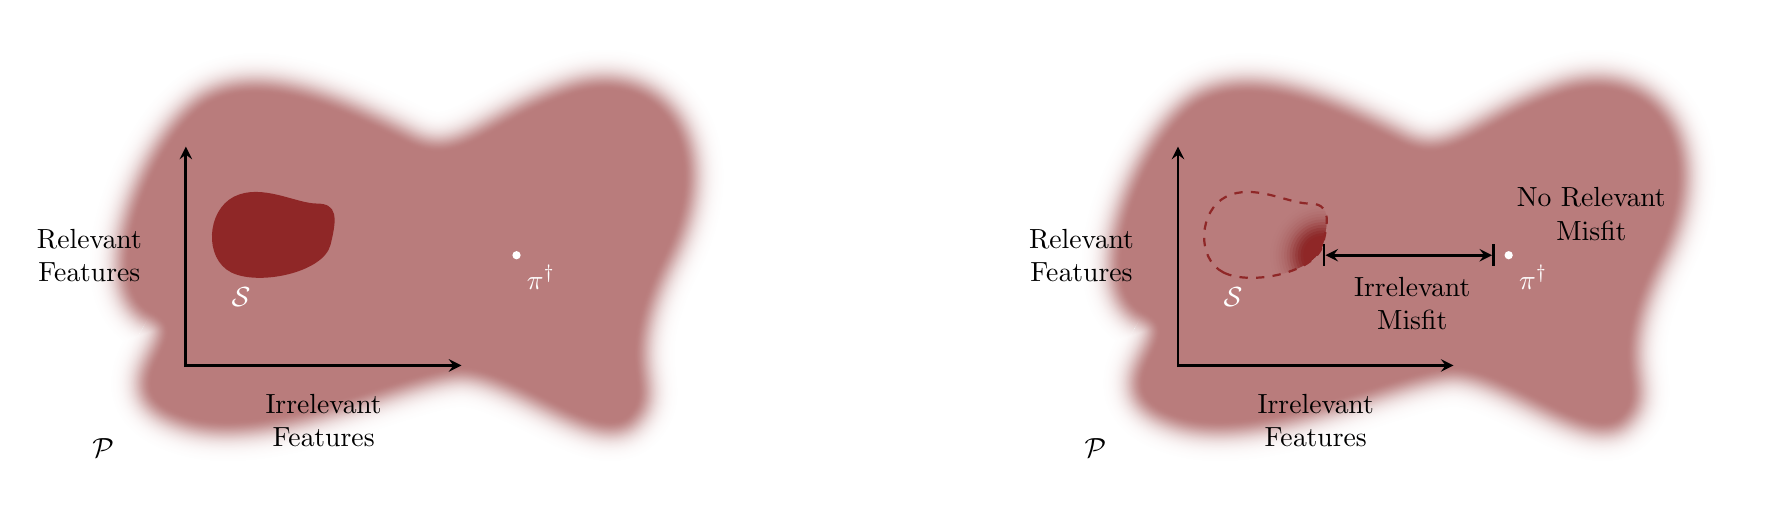
\begin{tikzpicture}[scale=0.35, thick] 

 \pgfmathsetmacro{\dx}{-18}
 \foreach \i in {1, 0.99, ..., 0} {
   \pgfmathsetmacro{\prop}{100 * exp(-5.0 * \i * \i)};
   \colorlet{custom}{mid!\prop!white};
   \draw[line width={30 * \i}, color=custom] 
     (-9.2 + \dx, -2) 
     .. controls (-11.2 + \dx, -1) and (-9 + \dx, 4.5) .. (-7 + \dx, 5.5) 
     .. controls (-5 + \dx, 6.5) and (-2 + \dx, 5) .. (0 + \dx, 4)
     .. controls (2 + \dx, 3) and (3 + \dx, 4.75) .. (6 + \dx, 5.75) 
     .. controls (9 + \dx, 6.75) and (11.25 + \dx, 4) .. (9.25 + \dx, 0)
     .. controls (7.25 + \dx, -4) and (9 + \dx, -4.75) .. (8 + \dx, -5.75) 
     .. controls (7 + \dx, -6.75) and (4 + \dx, -4) .. (2 + \dx, -4)
     .. controls (0 + \dx, -4) and (-5 + \dx, -6.75) .. (-8 + \dx, -5.75) 
     .. controls (-11 + \dx, -4.75) and (-7.2 + \dx, -3) .. (-9.2 + \dx, -2);
  }
  
  \fill [color=mid] (-9.2 + \dx, -2) 
    .. controls (-11.2 + \dx, -1) and (-9 + \dx, 4.5) .. (-7 + \dx, 5.5) 
    .. controls (-5 + \dx, 6.5) and (-2 + \dx, 5) .. (0 + \dx, 4)
    .. controls (2 + \dx, 3) and (3 + \dx, 4.75) .. (6 + \dx, 5.75) 
    .. controls (9 + \dx, 6.75) and (11.25 + \dx, 4) .. (9.25 + \dx, 0)
    .. controls (7.25 + \dx, -4) and (9 + \dx, -4.75) .. (8 + \dx, -5.75) 
    .. controls (7 + \dx, -6.75) and (4 + \dx, -4) .. (2 + \dx, -4)
    .. controls (0 + \dx, -4) and (-5 + \dx, -6.75) .. (-8 + \dx, -5.75) 
    .. controls (-11 + \dx, -4.75) and (-7.2 + \dx, -3) .. (-9.2 + \dx, -2);
    
  \node [] at (-11 + \dx, -7) { $\mathcal{P}$ };
    
  \pgfmathsetmacro{\ddx}{-3}
  \pgfmathsetmacro{\ddy}{0}
    
  \fill [color=dark] (-3.35 + \dx + \ddx, -0.625 + \ddy) 
    .. controls (-4.35 + \dx + \ddx, -0.125 + \ddy) and (-4.25 + \dx + \ddx, 1.625 + \ddy) .. (-3.25 + \dx + \ddx, 2.125 + \ddy) 
    .. controls (-2.25 + \dx + \ddx, 2.625 + \ddy) and (-1 + \dx + \ddx, 1.875 + \ddy) .. (-0.25 + \dx + \ddx, 1.875 + \ddy)
    .. controls (0.5 + \dx + \ddx, 1.875 + \ddy) and (0.5 + \dx + \ddx, 1.375 + \ddy) .. (0.25 + \dx + \ddx, 0.375 + \ddy)
    .. controls (0 + \dx + \ddx, -0.625 + \ddy) and (-2.35 + \dx + \ddx, -1.125 + \ddy) .. (-3.35 + \dx + \ddx, -0.625 + \ddy); 
  
  \node [color=white] at (-6 + \dx, -1.5) { $\mathcal{S}$ };
  
  \draw [->, >=stealth, line width=1, color=black] (-8 + \dx, -4) -- +(10, 0);
  \node[align=center] at (-3 + \dx, -6) { Irrelevant\\Features };
  
  \draw [->, >=stealth, line width=1, color=black] (-8 + \dx, -4.06) -- +(0, 8);
  \node[align=center] at (-11.5 + \dx, 0) { Relevant\\Features };
  
  \fill [fill=white] (4 + \dx, 0) circle (0.15)
  node [below right, color=white] { $\pi^{\dagger}$ };
  
  
 \pgfmathsetmacro{\dx}{+18}
 \foreach \i in {1, 0.99, ..., 0} {
   \pgfmathsetmacro{\prop}{100 * exp(-5.0 * \i * \i)};
   \colorlet{custom}{mid!\prop!white};
   \draw[line width={30 * \i}, color=custom] 
     (-9.2 + \dx, -2) 
     .. controls (-11.2 + \dx, -1) and (-9 + \dx, 4.5) .. (-7 + \dx, 5.5) 
     .. controls (-5 + \dx, 6.5) and (-2 + \dx, 5) .. (0 + \dx, 4)
     .. controls (2 + \dx, 3) and (3 + \dx, 4.75) .. (6 + \dx, 5.75) 
     .. controls (9 + \dx, 6.75) and (11.25 + \dx, 4) .. (9.25 + \dx, 0)
     .. controls (7.25 + \dx, -4) and (9 + \dx, -4.75) .. (8 + \dx, -5.75) 
     .. controls (7 + \dx, -6.75) and (4 + \dx, -4) .. (2 + \dx, -4)
     .. controls (0 + \dx, -4) and (-5 + \dx, -6.75) .. (-8 + \dx, -5.75) 
     .. controls (-11 + \dx, -4.75) and (-7.2 + \dx, -3) .. (-9.2 + \dx, -2);
  }
  
  \fill [color=mid] (-9.2 + \dx, -2) 
    .. controls (-11.2 + \dx, -1) and (-9 + \dx, 4.5) .. (-7 + \dx, 5.5) 
    .. controls (-5 + \dx, 6.5) and (-2 + \dx, 5) .. (0 + \dx, 4)
    .. controls (2 + \dx, 3) and (3 + \dx, 4.75) .. (6 + \dx, 5.75) 
    .. controls (9 + \dx, 6.75) and (11.25 + \dx, 4) .. (9.25 + \dx, 0)
    .. controls (7.25 + \dx, -4) and (9 + \dx, -4.75) .. (8 + \dx, -5.75) 
    .. controls (7 + \dx, -6.75) and (4 + \dx, -4) .. (2 + \dx, -4)
    .. controls (0 + \dx, -4) and (-5 + \dx, -6.75) .. (-8 + \dx, -5.75) 
    .. controls (-11 + \dx, -4.75) and (-7.2 + \dx, -3) .. (-9.2 + \dx, -2);
    
  \node [] at (-11 + \dx, -7) { $\mathcal{P}$ };
    
  \pgfmathsetmacro{\ddx}{-3}
  \pgfmathsetmacro{\ddy}{0}
    
  \draw [color=dark, dashed] (-3.35 + \dx + \ddx, -0.625 + \ddy) 
    .. controls (-4.35 + \dx + \ddx, -0.125 + \ddy) and (-4.25 + \dx + \ddx, 1.625 + \ddy) .. (-3.25 + \dx + \ddx, 2.125 + \ddy) 
    .. controls (-2.25 + \dx + \ddx, 2.625 + \ddy) and (-1 + \dx + \ddx, 1.875 + \ddy) .. (-0.25 + \dx + \ddx, 1.875 + \ddy)
    .. controls (0.5 + \dx + \ddx, 1.875 + \ddy) and (0.5 + \dx + \ddx, 1.375 + \ddy) .. (0.25 + \dx + \ddx, 0.375 + \ddy)
    .. controls (0 + \dx + \ddx, -0.625 + \ddy) and (-2.35 + \dx + \ddx, -1.125 + \ddy) .. (-3.35 + \dx + \ddx, -0.625 + \ddy); 
  
  \begin{scope}
    \clip (-3.35 + \dx + \ddx, -0.625 + \ddy) 
    .. controls (-4.35 + \dx + \ddx, -0.125 + \ddy) and (-4.25 + \dx + \ddx, 1.625 + \ddy) .. (-3.25 + \dx + \ddx, 2.125 + \ddy) 
    .. controls (-2.25 + \dx + \ddx, 2.625 + \ddy) and (-1 + \dx + \ddx, 1.875 + \ddy) .. (-0.25 + \dx + \ddx, 1.875 + \ddy)
    .. controls (0.5 + \dx + \ddx, 1.875 + \ddy) and (0.5 + \dx + \ddx, 1.375 + \ddy) .. (0.25 + \dx + \ddx, 0.375 + \ddy)
    .. controls (0 + \dx + \ddx, -0.625 + \ddy) and (-2.35 + \dx + \ddx, -1.125 + \ddy) .. (-3.35 + \dx + \ddx, -0.625 + \ddy);
    \foreach \i in {0, 0.05,..., 1} {
      \fill[opacity={exp(-5 * \i*\i)}, dark] (-2.75 + \dx, 0) circle ({2 * \i});      
    }
  \end{scope}
  
  \node [color=white] at (-6 + \dx, -1.5) { $\mathcal{S}$ };
  
  \draw [|<->|, >=stealth, line width=1, color=black] (-2.75 + \dx, 0) -- (3.5 + \dx, 0);
  \node[align=center] at (0.5 + \dx, -1.75) { Irrelevant\\Misfit };

  \node[align=center] at (7 + \dx, 1.5) { No Relevant\\Misfit };
  
  \draw [->, >=stealth, line width=1, color=black] (-8 + \dx, -4) -- +(10, 0);
  \node[align=center] at (-3 + \dx, -6) { Irrelevant\\Features };
  
  \draw [->, >=stealth, line width=1, color=black] (-8 + \dx, -4.06) -- +(0, 8);
  \node[align=center] at (-11.5 + \dx, 0) { Relevant\\Features };
  
  \fill [fill=white] (4 + \dx, 0) circle (0.15)
  node [below right, color=white] { $\pi^{\dagger}$ };
  
\end{tikzpicture}

\end{document}   